\documentclass[12pt]{article}
\usepackage[utf8]{inputenc}
\usepackage[a4paper]{geometry}
\usepackage{graphicx}
\usepackage{amsmath}
\usepackage[section]{placeins}
\usepackage{subcaption}
\usepackage[backend=bibtex]{biblatex}

\addbibresource{references.bib}

\title{COMP6212 Assignment 4}
\author{James Robinson}

\begin{document}

  \maketitle

  \section{Implementation of Kalman filter}

  The variance of the residual of a third-order autoregressive model of the time series data is calculated using MATLAB functions \texttt{m = ar(ts, 3); R = m.NoiseVariance;} where \texttt{ts} is a column vector of time series data. This value is used as an estimate of the observation noise variance $R$ in the Kalman filter. An initial estimate $\Theta(0)$ of the AR model weights is calculated as \texttt{(m.a(2:4) * -1)'}.

  For all values $n \in 4..N$, $\Theta(n | n)$, $P(n | n)$ (the error covariance) and $e(n)$ (the residual) are calculated as follows \cite{Kalman1960}:

  \begin{equation}
    \Theta(n | n - 1) = \Theta(n - 1 | n - 1)
  \end{equation}
  \begin{equation}
    Q = \alpha I
  \end{equation}
  \begin{equation}
    e(n) = y(n) - \Theta(n | n - 1)^T x(n)
  \end{equation}
  \begin{equation}
    K(n) = \frac{P(n | n - 1)x(n)}{R + x(n)^T P(n|n - 1) x(n)}
  \end{equation}
  \begin{equation}
    \Theta(n|n) = \Theta(n | n - 1) + K(n) e(n)
  \end{equation}
  \begin{equation}
    P(n | n) = (I - K(n)x(n)^T)P(n | n - 1)
  \end{equation}

  \section{Testing with artificial data}

  The Kalman filter implementation was first tested using artificial data. A time series of length 1000 was constructed with initial values at $n = 1..3$ of 2000 and $\Theta = \left(\begin{matrix}0.5 & 0.6 & -0.1\end{matrix}\right)^T$, with random variance from a 20dBW white Gaussian noise signal added at each step. The resulting time series is shown in figure~\ref{fig:artificial_ts}. A low process noise value of $\alpha = 0.000000001$ was selected for this test to prevent overfitting. The AR model parameters $\Theta$ over time, as calculated by the Kalman filter, are shown in figure~\ref{fig:artificial_theta}. As can be seen, the parameters immediately converge to match the parameters used in synthesis of the time series. The residual closely matches the deliberately introduced noise, as shown in figure~\ref{fig:artificial_residual}.

  \begin{figure}
    \centering
    \begin{subfigure}[b]{0.45\textwidth}
      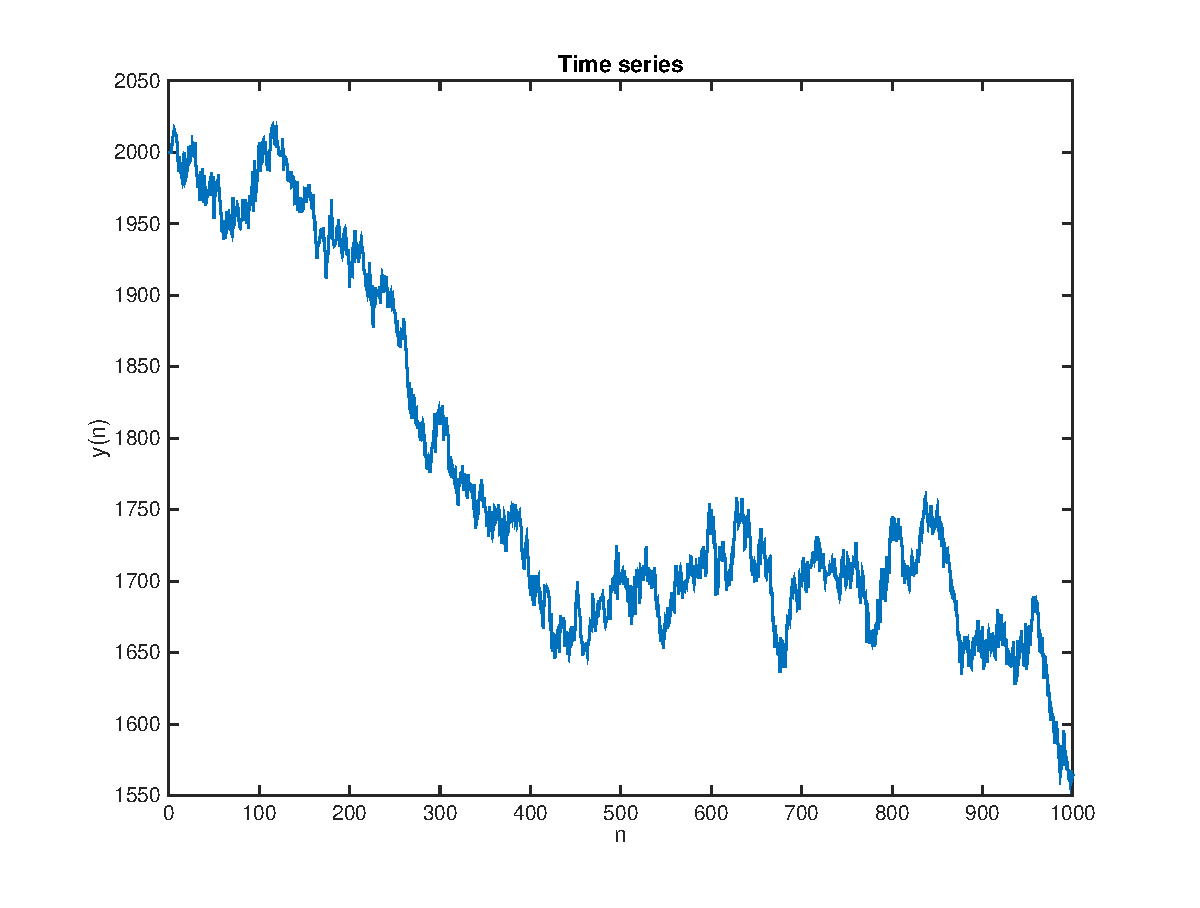
\includegraphics[width=\textwidth]{figures/artificial_ts.eps}
      \caption{Time series}
      \label{fig:artificial_ts}
    \end{subfigure}
    \begin{subfigure}[b]{0.45\textwidth}
      \includegraphics[width=\textwidth]{figures/artificial_theta.eps}
      \caption{AR weights over time ($\Theta$)}
      \label{fig:artificial_theta}
    \end{subfigure}
    \begin{subfigure}[b]{0.45\textwidth}
      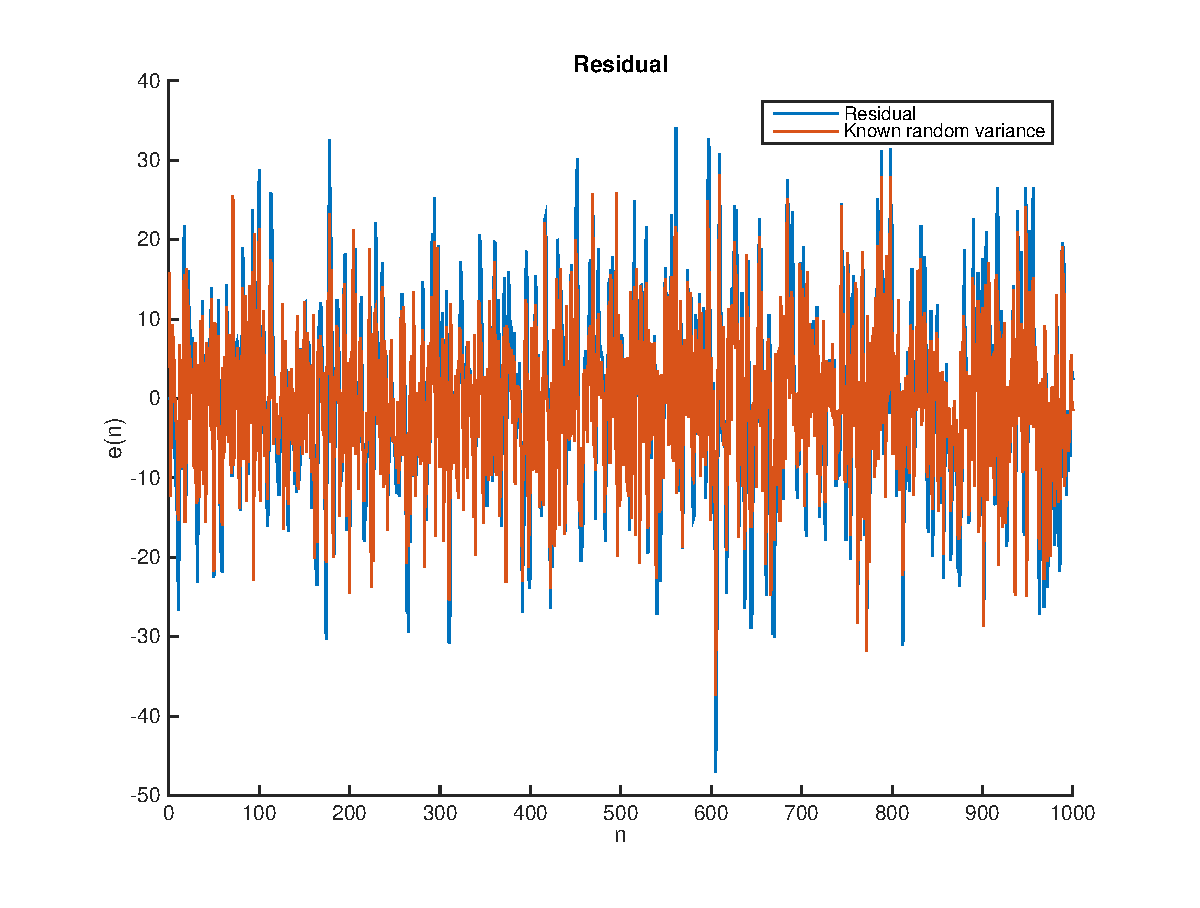
\includegraphics[width=\textwidth]{figures/artificial_residual.eps}
      \caption{Residual}
      \label{fig:artificial_residual}
    \end{subfigure}
    \caption{Kalman filtering of artificial time series data}
  \end{figure}

  \section{Results with S\&P 500 data}

  After verifying the correct function of the Kalman filter implementation, the filter was run on 20 years of monthly S\&P 500 index data (figure~\ref{fig:real_ts}). An optimisation step was used to select a value for the process noise variance $\alpha$ minimising the residual. A value that is too high causes overfitting, whereas a value that is too low prevents the Kalman filter from adjusting the AR model parameters at all. Figure~\ref{fig:alpha} shows the sum of the absolute residuals for values of $\alpha$ in the range $10^{-10}$ to 1. The minimum residual found at approximately $\alpha = 10^{-3}$, so this value was selected. The AR model parameters estimated by the Kalman filter are shown in figure~\ref{fig:real_theta}, and figure~\ref{fig:real_residual} shows the residual.

  \begin{figure}
    \centering
    \includegraphics[width=0.45\linewidth]{figures/alpha.eps}
    \caption{Optimising $\alpha$}
    \label{fig:alpha}
  \end{figure}

  \begin{figure}
    \centering
    \begin{subfigure}[b]{0.45\textwidth}
      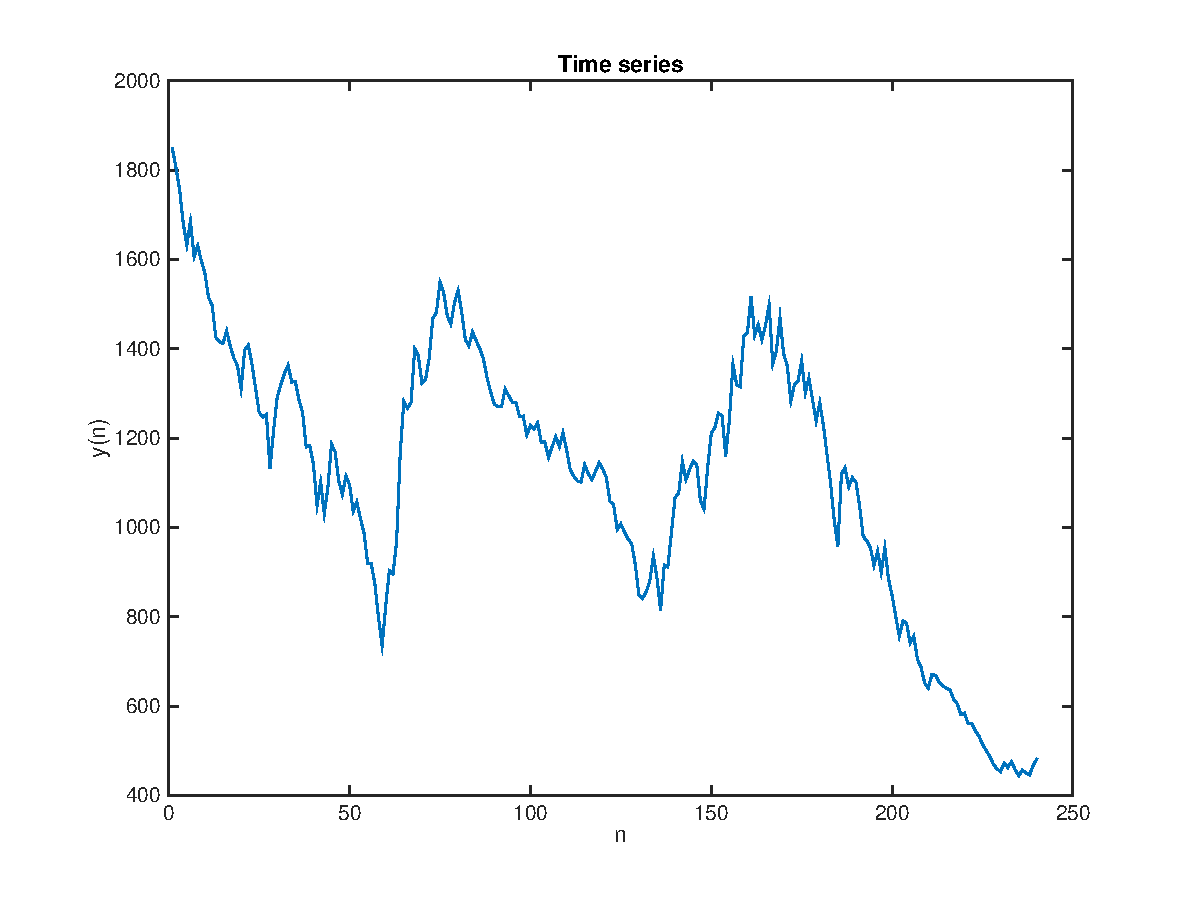
\includegraphics[width=\textwidth]{figures/real_ts.eps}
      \caption{Time series}
      \label{fig:real_ts}
    \end{subfigure}
    \begin{subfigure}[b]{0.45\textwidth}
      \includegraphics[width=\textwidth]{figures/real_theta.eps}
      \caption{AR weights over time ($\Theta$)}
      \label{fig:real_theta}
    \end{subfigure}
    \begin{subfigure}[b]{0.45\textwidth}
      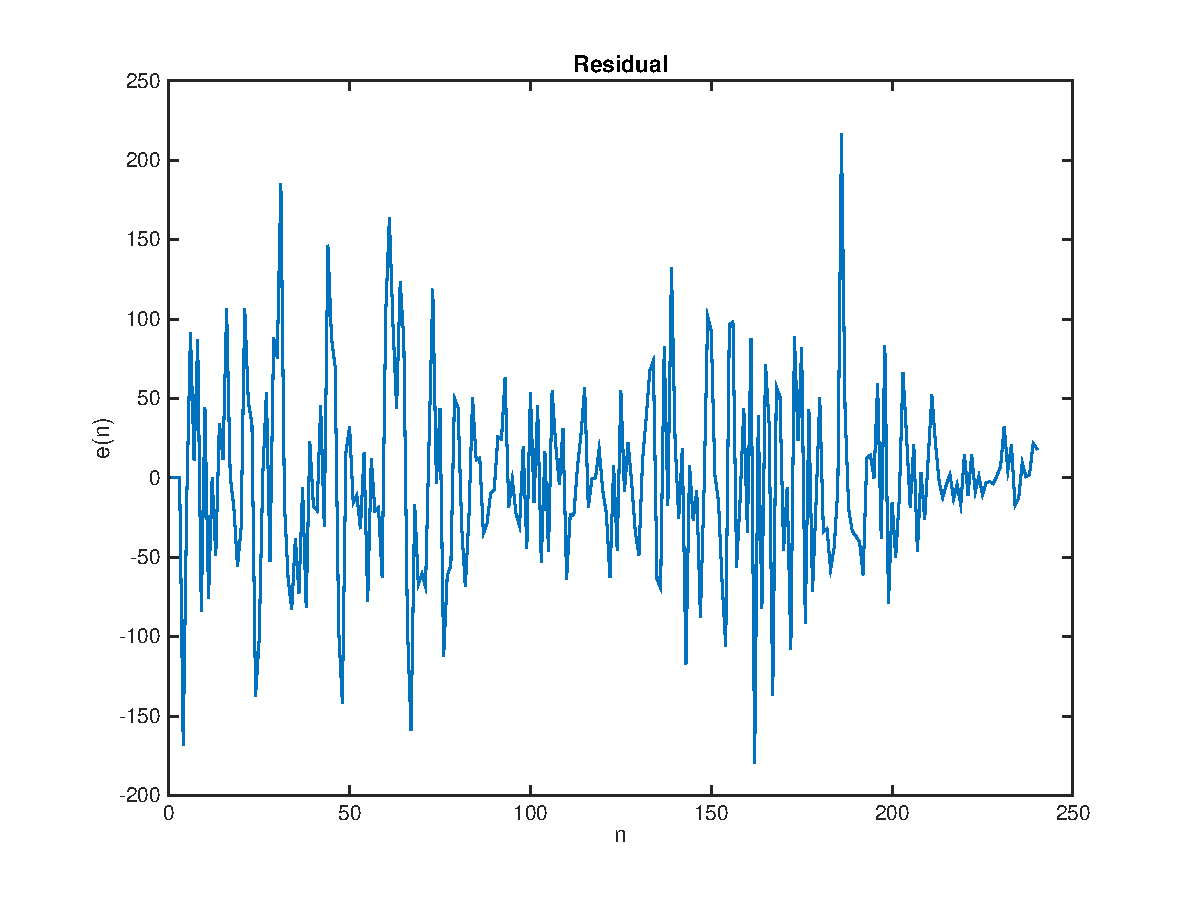
\includegraphics[width=\textwidth]{figures/real_residual.eps}
      \caption{Residual}
      \label{fig:real_residual}
    \end{subfigure}
    \caption{Kalman filtering of S\&P 500 time series data}
  \end{figure}

  \section{Fitting the residual}

  Time series data for the following variables was obtained, and bicubic interpolation was used to fill in missing data for datasets shorter than the S\&P index data.

  \begin{itemize}
    \item Spot Oil Price, West Texas Intermediate, in dollars per barrel (OIL)
    \item NAPM, ISM Manufacturing, Purchasing Managers' Composite Index (PMI)
    \item Disposable Personal Income per capita (INCOME)
    \item Corporate Profits After Tax (CORP\_PROFIT)
    \item US Population (POPULATION)
    \item US Unemployment rate (UNEMPLOYED)
  \end{itemize}

  Lasso regularization \cite{Tibshirani1996} was used to fit these variables to the residual. The CVX library was used to optimise the following objective function, where $e$ is the residual (a Tx1 vector), $R$ is a matrix containing time series for each variable (TxN), $w$ is a column vector of weights (Nx1), and $\tau$ is the regularisation parameter controlling sparsity.

  \begin{equation}
    \min \left|\left|e - Rw\right|\right|_2^2 + \tau\left|\left|w\right|\right|_1
  \end{equation}

  After experimentation, a value of $\tau = 1.3$ was chosen in order to select exactly 3 variables. The calculated weights of these variables are shown in figure~\ref{fig:weights}, and the time series $Rw$ resulting from multiplying the variables by the weights is shown in figure~\ref{fig:weighted_variables}, plotted against the residual.

  \begin{figure}
    \centering
    \begin{subfigure}[b]{0.45\textwidth}
      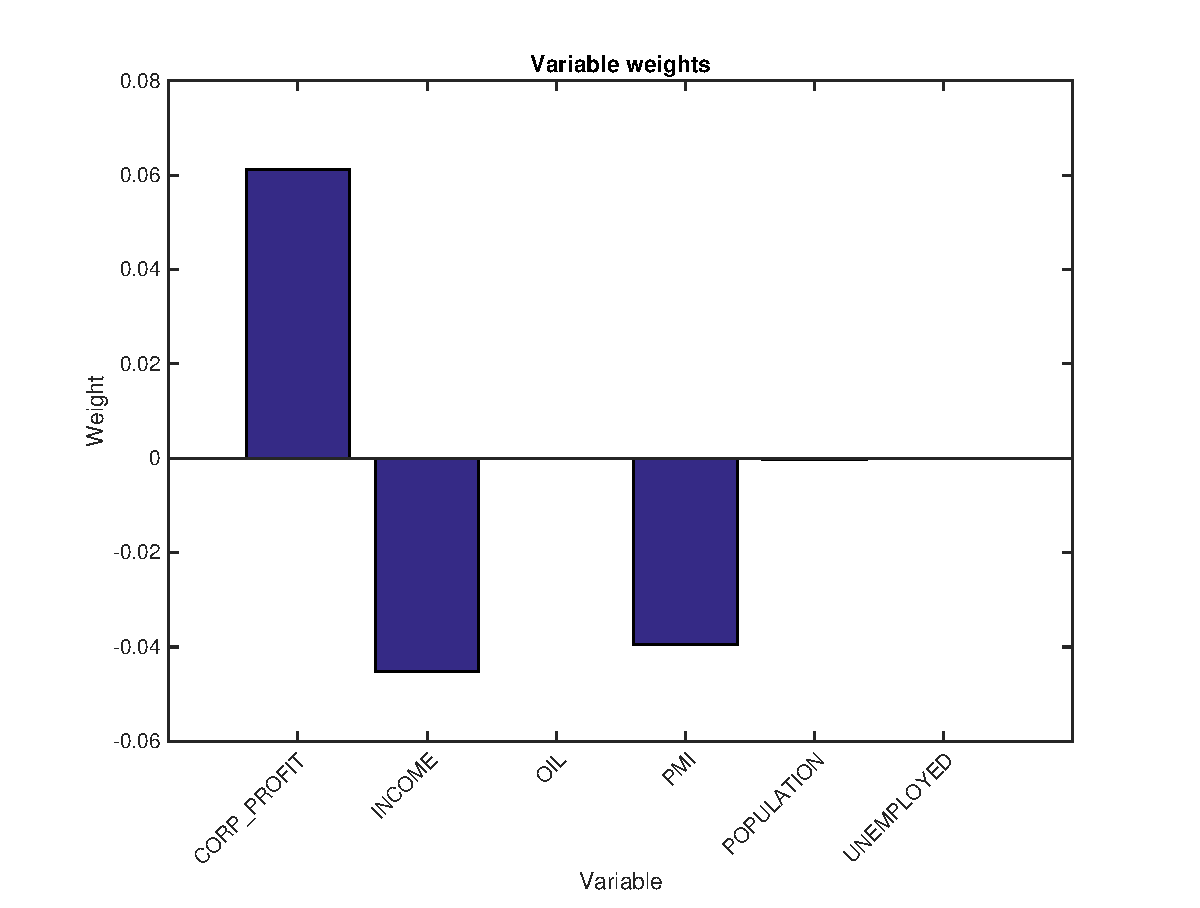
\includegraphics[width=\textwidth]{figures/weights.eps}
      \caption{Weights}
      \label{fig:weights}
    \end{subfigure}
    \begin{subfigure}[b]{0.45\textwidth}
      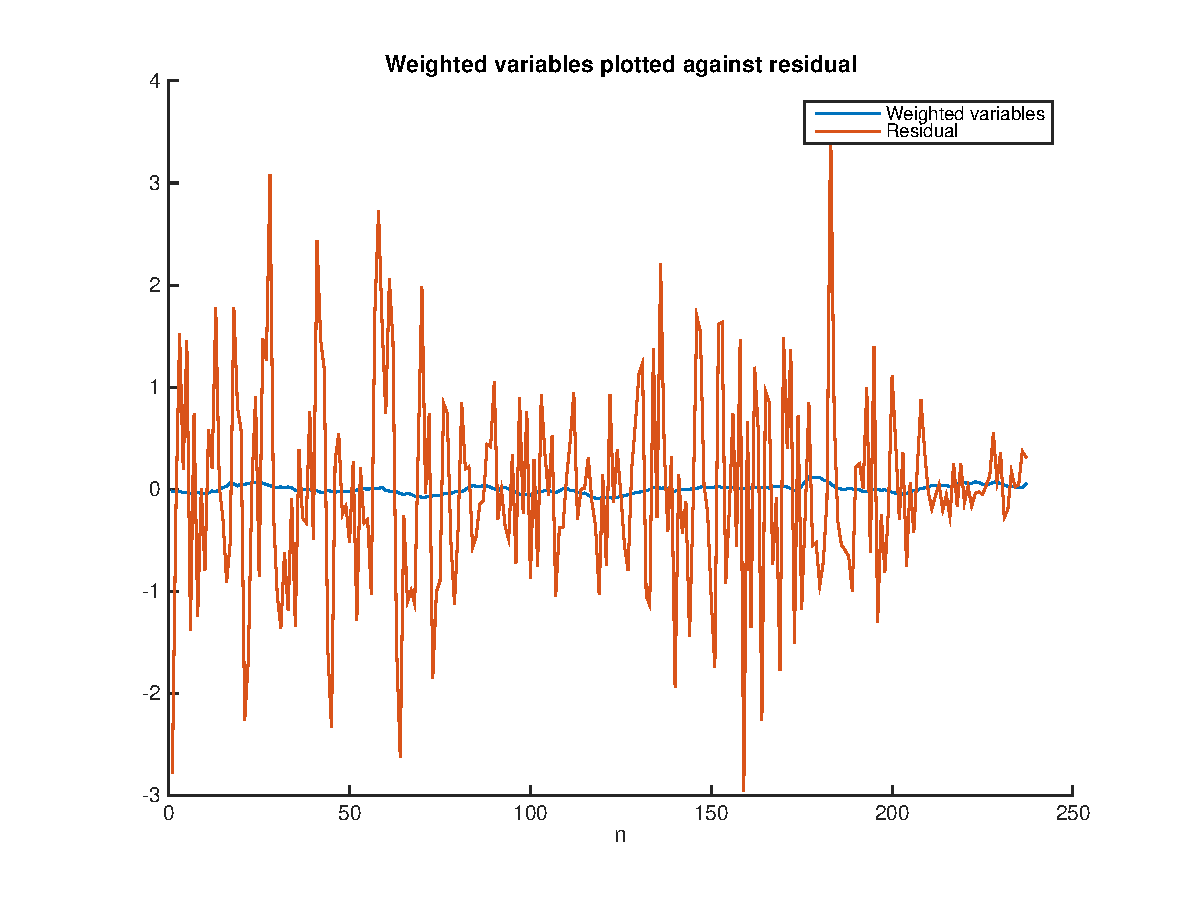
\includegraphics[width=\textwidth]{figures/weighted_variables.eps}
      \caption{Weighted variables}
      \label{fig:weighted_variables}
    \end{subfigure}
    \caption{Fitting variables to the residual using Lasso}
  \end{figure}

  \section{Stochastic volatility}

  A stochastic volatility model is a stochastic model in which the variance is also randomly distributed. Stochastic volatility models resolve one shortcoming of the Black-Scholes model: the Black-Scholes model assumes that the underlying volatility is constant over the life of an option, and unaffected by changes in the underlying asset price. By assuming that the volatility of the underlying price is also randomly distributed, it is possible to model options prices more accurately than the Black-Scholes model.

  Starting with a constant volatility, it is assumed that the option's underlying asset price follows geometric Brownian motion:

  \begin{equation}
    dS_t = \mu S_t\,dt + \sigma S_t\,dW_t
  \end{equation}

  where $\mu$ is the expected return of $S_t$, $\sigma$ is the constant volatility, and $dW_t$ is a standard Weiner process (random walk) with a mean of 0 and variance of 1. This basic model with constant volatility forms the basis of non-stochastic volatility models including the Black-Scholes model.

  In a stochastic volatility model, the constant volatility $\sigma$ is replaced with a function $v_t$ which models the variance of $S_t$:

  \begin{equation}
    dS_t = \mu S_t\,dt + \sqrt{\nu_t} S_t\,dW_t
  \end{equation}
  \begin{equation}
    d\nu_t = \alpha_{S,t}\,dt + \beta_{S,t}\,dB_t
  \end{equation}

  A popular stochastic volatility model is the Heston model \cite{Heston1993}, which ``derive[s] a closed-form solution for the price of a European call option on an asset with stochastic volatility''. Due to space constraints, the details cannot be reproduced here.

  \printbibliography

\end{document}
